\documentclass[t,ignorenonframetext]{beamer}
\mode<presentation> {
  \usetheme{PaloAlto}
  %\usecolortheme{seagull}
  %\usefonttheme{serif}
}

\usefonttheme{structuresmallcapsserif}
\usepackage{enumerate,graphicx}
\usepackage[]{textpos}
\usepackage{comment}
\usepackage{algorithm}
\usepackage{caption}
\usepackage{framed}
\usepackage[noend]{algorithmic}
\usepackage{ragged2e}
\usepackage{svg}
%\definecolor{green}{rgb}{0.53, 0.66, 0.42}
\definecolor{red}{rgb}{0.8, 0.0, 0.0}


\definecolor{brown}{RGB}{139, 137, 137}
\definecolor{maroon}{RGB}{178, 34, 34}
\definecolor{green}{RGB}{34, 139, 34}
\definecolor{types}{RGB}{72, 61, 139}

\newcommand{\intn}[1]{\ensuremath{\tt {\color{brown} int#1\xspace}}}
\newcommand{\rndn}[1]{\ensuremath{\tt {\color{brown} rnd#1\xspace}}}
\newcommand{\struct}[0]{\ensuremath{\tt {\color{blue} struct~}}}
\newcommand{\public}[0]{\ensuremath{\tt {\color{maroon} public~}}}
\newcommand{\secure}[0]{\ensuremath{\tt {\color{maroon} secure~}}}
\newcommand{\at}[1]{\ensuremath{\tt {\color{green} @#1}}}
\newcommand{\bit}[1]{\ensuremath{\tt {\color{green} #1\xspace}}}
\newcommand{\types}[1]{{\tt {\color{types} <#1>}}}
\newcommand{\type}[1]{{\tt {\color{types} #1}}}
\newcommand{\while}[0]{\ensuremath{\tt {\color{blue} while~}}}
\newcommand{\bound}[1]{\ensuremath{\tt {\color{blue} bfor}(#1)}}
\newcommand{\for}[0]{\ensuremath{\tt {\color{blue} for~}}}
\newcommand{\ifs}[0]{\ensuremath{\tt {\color{blue} if~}}}
\newcommand{\then}[0]{\ensuremath{\tt {\color{blue} then~}}}
\newcommand{\elses}[0]{\ensuremath{\tt {\color{blue} else~}}}
\newcommand{\return}[0]{\ensuremath{\tt {\color{blue} return~}}}
\newcommand{\define}[0]{\ensuremath{\tt {\color{blue} define~}}}
\newcommand{\typedef}[0]{\ensuremath{\tt {\color{blue} typedef~}}}
\newcommand{\native}[0]{\ensuremath{\tt {\color{blue} native~}}}
\newcommand{\partf}[0]{\ensuremath{\tt {\color{blue} phantom~}}}
\newcommand{\dummy}[0]{\ensuremath{\tt {\color{blue} dummy~}}}
\newcommand{\func}[1]{\ensuremath{\tt {\color{orange} #1}}}

%\usepackage[usenames, dvipsnames]{color}
%\usepackage{vplace}
\DeclareCaptionFormat{myformat}{#3}
\captionsetup[algorithm]{format=myformat}
%\usepackage{algpseudocode}
%\usepackage{algorithmicx,color,xspace,xcolor,fullpage,url}
\setlength{\TPHorizModule}{5mm}
\setlength{\TPVertModule}{\TPHorizModule}

% The line below is what I talked about that makes all
% items in a list into overlays
%\beamerdefaultoverlayspecification{<+->}
\newcommand{\tc}[1]{$\backslash$\texttt{#1}}
\newcommand{\kartik}[1]{{\footnotesize\color{blue}[Kartik: #1]}}
\newcommand\myblock[4]{%
\begin{textblock}{#1}(#2, #3)%
  \begin{center}
    #4
  \end{center}
\end{textblock}
}
\newcommand\rightblock[4]{%
\begin{textblock}{#1}(#2, #3)%
  \begin{flushright}
    #4
  \end{flushright}
\end{textblock}
}
\newcommand\leftblock[4]{%
\begin{textblock}{#1}(#2, #3)%
  \vspace*{\fill}
    #4
  \vspace*{\fill}
\end{textblock}
}
%\algtext*{EndWhile}% Remove "end while" text
%\algtext*{ENDIF}% Remove "end if" text

\title[]{{\tt iDASH} - Secure Genome Analysis Competition Using {\tt ObliVM}}
\author[]{Xiao Shaun Wang, Chang Liu, \textbf{Kartik Nayak}, Yan Huang and Elaine Shi}
\date{University of Maryland, College Park\\Indiana University, Bloomington}
\begin{document}
\frame{
\maketitle
}

\section{{\tt ObliVM}}

\begin{frame}[fragile]{{\tt ObliVM}}

\myblock{20}{0}{1}{
\LARGE{Programming Framework for Secure Computation}
}
\pause
\leftblock{20}{0}{6}{
{\color{green}{ \Large Ease-of-use:} } easy for non-specialist programmers to use
}
\pause
\leftblock{20}{0}{8}{
{\color{green}{\Large Efficiency:} } compiles programs to \emph{small} circuits
}

\end{frame}

\begin{frame}

\begin{figure}[H]
        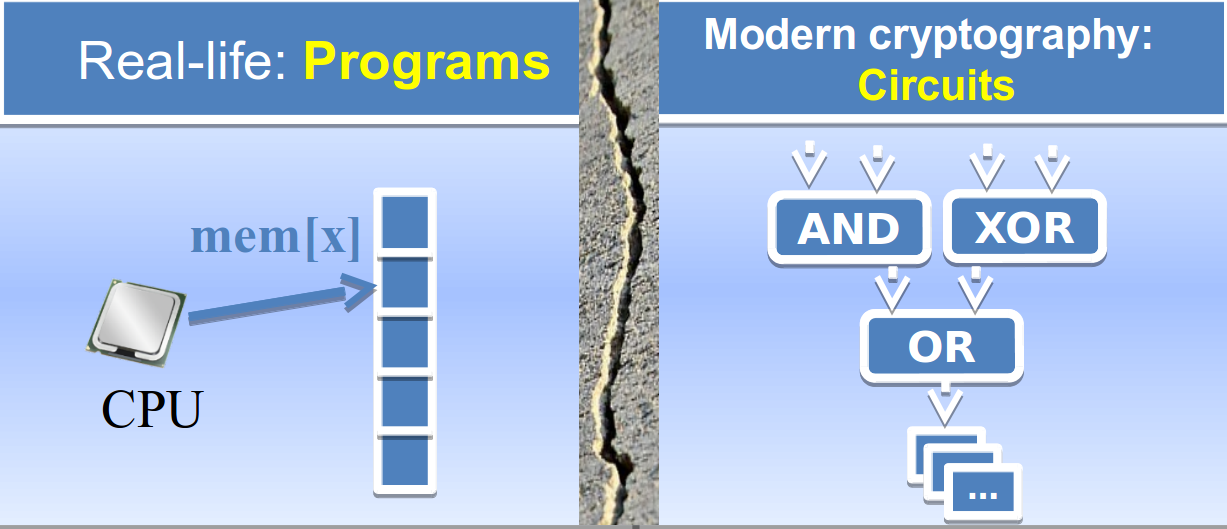
\includegraphics[width=\textwidth]{circuit}
      \end{figure}

\end{frame}

\begin{frame}[fragile]{{\tt ObliVM}}

\myblock{20}{0}{1}{
\LARGE{Programming Framework for Secure Computation}
}

\leftblock{20}{0}{6}{
{\color{green}{ \Large Ease-of-use:} } easy for non-specialist programmers to use
}

\leftblock{20}{0}{8}{
{\color{green}{\Large Efficiency:} } compiles programs to \emph{small} circuits
}

\leftblock{20}{0}{10}{
{\color{green}{\Large Formal Security:} } type system is being formalized
}
\myblock{20}{0}{12}{
{\LARGE{\url{http://oblivm.com}}}
}

\end{frame}
\section{Task 1A}

\begin{comment}
\begin{frame}{Compute MAF}
\begin{itemize}
\item Compute minor allele frequencies
\myblock{10}{0}{1}{\textbf{Alice}%\\
%$l^A = (e^A_1,...,e^A_n)$
}
\myblock{10}{10}{1}{\textbf{Bob}%\\
%$l^B = (e^B_1,...,e^B_n)$
}
\leftblock{21}{0}{12}{
  \footnotesize{\color{green}Cleartext}\\
  \footnotesize{\color{red}Secure}
}
%\pause
%\myblock{20}{0}{4}{where $e_i^X \in \{A, T, C, G\}$}
%\pause
\myblock{10}{0}{2}{
\color{blue}{AA AC AA}\\
\color{green}{$f_A^{Alice} = 5, f_C^{Alice} = 1$}
}
\myblock{10}{10}{2}{
\color{blue}{AA AC CC}\\
{\color{green}$f_A^{Bob} = 3, f_C^{Bob} = 3$}
}
\pause
\myblock{20}{0}{5}{
Compute $min(f^{Alice}_A + f^{Bob}_A, f^{Alice}_C+f^{Bob}_C)$
}
\pause
\myblock{20}{0}{7}{
Secure Computation:
{\color{red}$MAF = min(f^{Alice}_A + f^{Bob}_A, f^{Alice}_C+f^{Bob}_C)$}\\
%\pause
%40 AND gates
}
\end{itemize}
\end{frame}

\begin{frame}{Code in {\tt ObliVM-lang}: Compute MAF }
\begin{figure}[H]
\includegraphics[width=\textwidth]{1aa}
%\caption{Code for Task 1a written in {\tt ObliVM-lang}}
\end{figure}
\end{frame}

\section{Task 1B}
\label{sec:task1b}

\begin{frame}{Problem Statement: Compute $\chi^2$ statistic}
  \begin{itemize}
    \item Task 1b: Computing $\chi^2$ statistic
    \myblock{10}{0}{1}{\textbf{Alice}\\
      Case: {\color{blue} AA AC AA}\\
      Control: {\color{blue} AA CA CA}
    %   List of case and control alleles
    %  $l^A_{case} = (e^A_1,...,e^A_n)$\\
    %  $l^A_{control} = (e'^A_1,...,e'^A_n)$
    }
    \myblock{10}{10}{1}{\textbf{Bob}\\
      Case: {\color{blue} AA AC CC}\\
      Control: {\color{blue} CA AC CC}
    %  $l^B_{case} = (e^B_1,...,e^B_n)$\\
    %  $l^B_{control} = (e'^B_1,...,e'^B_n)$
    }
    \leftblock{21}{0}{11}{
      \footnotesize{\color{green}Cleartext}\\
      \footnotesize{\color{red}Secure}
    }
    \pause
    \leftblock{20}{0}{5}{
      $a, b$: allele counts for case group \\%in $l_{case} = l^A_{case} || l^B_{case}$\\
      $c, d$: allele counts for control group \\%in $l_{control} = l^A_{control} || l^B_{control}$
      (similar to Task 1A)
    }
    \pause
    \myblock{20}{0}{8}{
      {\color{red} $\chi^2 = n\times\frac{(ad-bc)^2}{rsgk}$}\\
      where $r = a + b, s = c + d, g = a + c,$\\$k = b + d, n =  r + s$
    }
  \end{itemize}
\end{frame}

%\begin{frame}{Solution: Compute $\chi^2$ statistic}
%    \leftblock{20}{0}{1}{
%      $a, b$: frequencies of two alleles in $l_{case} = l^A_{case} || l^B_{case}$\\
%      $c, d$: frequencies of two alleles in $l_{control} = l^A_{control} || l^B_{control}$
%    }
%    \pause
%  \vspace{12mm}
%  \begin{itemize}
%    \item Compute partial values: {\color{green}\\$a^A,b^A,c^A,d^A$ for Alice \\$a^B,b^B,c^B,d^B$ for Bob}
%      \pause
%    \item In Secure Computation, {\color{red} compute $a = a^A + a^B$ \ldots}
%  \end{itemize}
%  \myblock{20}{0}{1}{
%    {\color{red} $\chi^2 = n\times\frac{(ad-bc)^2}{rsgk}$}
%  }
%\end{frame}

\begin{frame}{Results: Compute $\chi^2$ statistic}
  \begin{itemize}
    \item Floating point computation %\kartik{number of bits used}
    \item Absolute accuracy\\
      $1.11 \times 10^{-4}$ with 7763 gates\\
      $5.6 \times 10^{-8}$ with 14443 gates
  \end{itemize}
\end{frame}

\begin{frame}{Code in {\tt ObliVM-lang}: Compute $\chi^2$ statistic }
\begin{figure}[H]
\includegraphics[width=\textwidth]{1b}
%\caption{Code for Task 1b written in {\tt ObliVM-lang}}
\end{figure}
\end{frame}

\section{Set union}
\label{sec:setunion}

\begin{frame}{Building Block: Secure Set Union}
  \myblock{10}{0}{0}{\textbf{Alice}\\
      $S^A$\\
      \color{blue}{\{a, b, c\}}
    }
    \myblock{10}{10}{0}{\textbf{Bob}\\
      $S^B$\\
      \color{blue}{\{b, d, e\}}
    }
    \pause
    \myblock{20}{0}{3.5}{Cardinality of the union of the sets i.e. $|S^A \cup S^B|$\\
\color{blue}{$|S^A \cup S^B| = 5$}}
    \pause
    \rightblock{21}{0}{-1}{
      \footnotesize{\color{green}Cleartext}\\
      \footnotesize{\color{red}Secure}
    }
    \leftblock{20}{0}{8}{Strawman solution:}
    \rightblock{20}{0}{12}{$O(N \log^2 N)$}
    \vspace{40mm}
    \begin{algorithm}[H]
      \begin{algorithmic}[1]
        \STATE {\color{red} Sort the combined array $S^A || S^B$ obliviously}
        \pause
        \STATE {\color{red} Compute cardinality in a single pass}
      \end{algorithmic}
      \caption{union($S^A, S^B$)}
    \end{algorithm}
\end{frame}

\begin{frame}{Set Union: Oblivious Merge}
  \leftblock{21}{0}{13}{
      \footnotesize{\color{green}Cleartext}\\
      \footnotesize{\color{red}Secure}
    }
  \begin{algorithm}[H]
      \begin{algorithmic}[1]
        \STATE {\color{green} Local sort of $S^A$ and $S^B$}
        \pause
        \STATE {\color{red} Oblivious merge of sorted lists}
        \pause
        \STATE {\color{red} Compute cardinality in a single pass}
      \end{algorithmic}
      \caption{union($S^A, S^B$)}
    \end{algorithm}
    \rightblock{20}{0}{-1}{$O(N \log N)$}
\end{frame}

\begin{frame}{Code: Oblivious Merge}
  \begin{figure}[H]
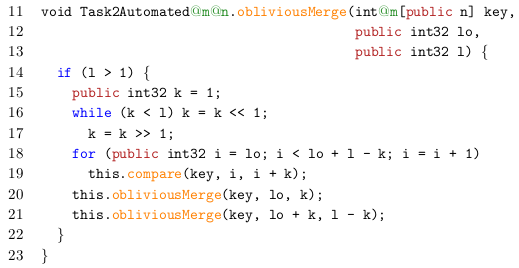
\includegraphics[width=\textwidth]{oblivous_merge}
%\caption{Code for Task 1b written in {\tt ObliVM-lang}}
\end{figure}
\end{frame}
\begin{frame}[fragile]{Set Union: Bloom Filter}
  \begin{itemize}
    \item Common case: Check for existence of elements
    \item Our case: Approximate the cardinality of a set $S$
  \end{itemize}
  \only<1>{
      \begin{figure}[H]
        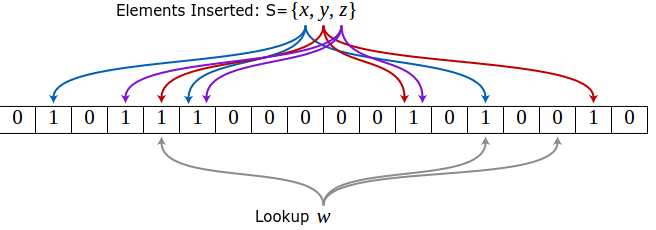
\includegraphics[width=0.8\textwidth]{bloom_filter}
      \end{figure}
      }
      \only<2>{
      \myblock{20}{0}{2}{
        \LARGE{$|S|_{MLE} = \frac{\ln(1-\frac{X}{m})}{k\ln(1-1/m)}$}
      }
      \pause
      \leftblock{20}{0}{6}{
        where\\ $X$: number of bits set,\\ $m$: number of bits in the bloom filter, \\
        $k$: number of hash functions,\\ $|S|_{MLE}$: maximum likelihood estimate of $|S|$
      }
      }
\end{frame}

\begin{frame}{Set Union: Bloom Filter}
  \leftblock{21}{0}{13}{
      \footnotesize{\color{green}Cleartext}\\
      \footnotesize{\color{red}Secure}
    }
  \begin{algorithm}[H]
      \begin{algorithmic}[1]
        \STATE {\color{green} Compute bloom filters locally}
        \pause
        \STATE {\color{red} In secure computation, compute bitwise OR and count number of 1's}
        \pause
        \STATE {\color{green} Compute estimated $|S|$ in cleartext}
        %http://www.l3s.de/~papapetrou/publications/Bloomfilters-DAPD.pdf
      \end{algorithmic}
      \caption{union($S^A, S^B$)}
    \end{algorithm}
  %\begin{itemize}
  %  \item {\color{green} Compute bloom filters locally}
    %\kartik{image for local computation}
  %  \pause
  %  \item {\color{red} In secure computation, Compute bitwise OR and count number of 1's}
  %  \pause
  %  \item {\color{green} Compute $|S|$ in cleartext}
  %\end{itemize}
  \pause
      \rightblock{20}{0}{0}{$O(m)$ operations, $m$: number of bits used for bloom filter\\
      $m = O(N)$, number of elements inserted in the bloom filter}
\end{frame}

\begin{frame}{Code: CountOnes}
  \begin{figure}[H]
        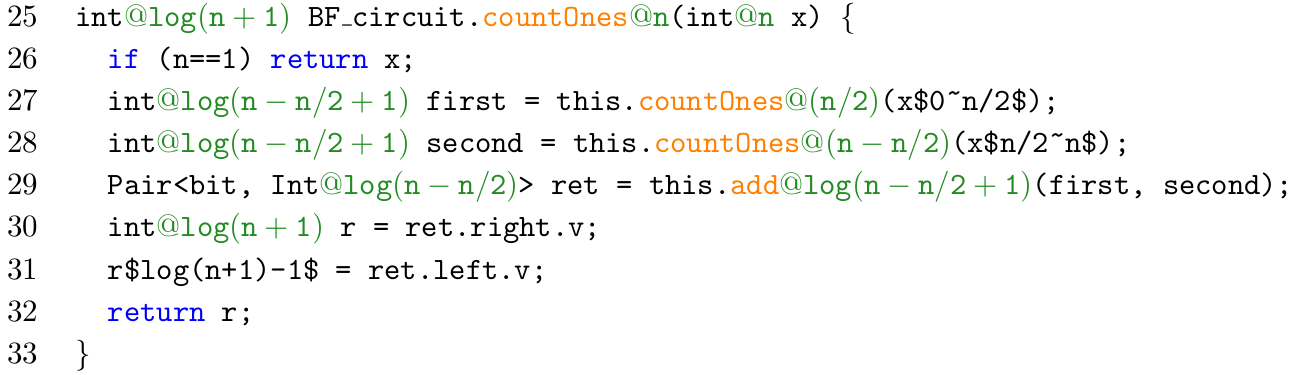
\includegraphics[width=\textwidth]{count_ones}
      \end{figure}
\end{frame}
%\begin{frame}
%  relative errors?
%\end{frame}

\section{Task 2A}
\label{sec:task1b}


\begin{frame}{Problem Statement: Hamming Distance}
Alice and Bob maintain records of type $(ref, svtype, alt)$ that differ from the reference
  \begin{framed}
{\tt~\\
d = 0;\\
for each record of type SNP or SUB\\
\qquad  if ((x == null) || (y == null) || (x.ref == y.ref \&\& x.alt != y.alt)\\
\qquad    d += 1;\\
end for\\
}
\end{framed}
\end{frame}

\begin{frame}{Solution: Hamming Distance}
  \myblock{10}{0}{0}{Alice
    }
    \myblock{10}{10}{0}{Bob
    }

    \myblock{10}{0}{2}{
      \footnotesize{\color{blue}{$S^A = $\{(1, T, SNP),(75, G, SNP)\}}}\\
      \footnotesize{\color{blue}{}}
    }
    \myblock{10}{10}{2}{
      \footnotesize{\color{blue}{$S^B = $\{(1, T, SNP),(18, A, SNP)\}}}
    }
    \myblock{20}{0}{4}{We need all positions that have been modified, but not modified to the same value}
    \leftblock{20}{0}{7}{
      {\color{blue}Hamming Distance = $|S^A \cup S^B| - |S^A \cap S^B|$ = $|\{(75, G, SNP),(18, A, SNP)\}|$}
    }
    %\leftblock{20}{0}{10}{
    %  Compute $d1 - d2$
    %}
    %\myblock{20}{0}{5}{
    %  $|S^A\cup S^B|$ \pause $ - |S^A\cap S^B|$ \pause $ = 2\times|S^A\cup S^B|-|S^A| - |S^B|$
    %}
    %\myblock{20}{0}{7}{
    %  Compute $|S^A\cup S^B|$ as suggested earlier
    %}
\end{frame}

\section{Task 2B}
\label{sec:task2b}

\begin{frame}{Problem Statement: Edit Distance}
  Alice and Bob maintain records of type $(ref, svtype, alt)$ that differ from the reference
  \begin{framed}
{\tt
Replacement: Calculate like hamming distance\\
Insertion/Deletion:\\
\qquad If one party modifies a position, add len(alt) to edit distance\\
\qquad If both parties modify a position, add len(max(alt1, alt2)) to edit distance
}
\end{framed}
\end{frame}

\begin{frame}{Solution: Edit Distance}
%  \kartik{shoudl be replaced with an example, hard to follow}
%  \begin{itemize}
%    \item Alice computes $S_1^A = \{(ref, i), i \in [1, len(alt)] \forall (ref, svtype, alt)\}$. Similarly for Bob.
%    \item $d1 = |S_1^A \cup S_1^B|$: all the positions that have been modified
%    \item Alice computes $S_1^B = \{(ref,svtype, alt, i), i\in[1, len(alt)] \forall (ref, svtype, alt)\}$
%  \end{itemize}
  \myblock{10}{0}{0}{
      Alice\\
      \footnotesize{\color{blue}{\{(1, T, SNP),\\ (10, TCG, INS),\\ (75, G, SNP)\}}}\\
    }
    \myblock{10}{10}{0}{
      Bob\\
      \footnotesize{\color{blue}{\{(1, T, SNP),\\ (10, CA, INS),\\ (18, A, SNP)\}}}
    }
    \pause
    \leftblock{22}{0}{5}{
      \small{\color{blue}{$S_1^A = \{(1, 1),(10, 1),(10, 2),(10, 3),(75, 1)\}$ }}\\
      \small{\color{blue}{$S_2^A = \{(1, T, 1),(10, T, 1),(10, C, 2),(10, G, 3),(75, G, 1)\}$ }}\\
    }
    \pause
    \leftblock{22}{0}{9}{
      {\color{blue}$d1 = |S_1^A \cup S_1^B| = |\{(1, 1),(10, 1),(10, 2),(10, 3),(75, 1),(18, 1)\}|$}
    }
    \pause
    \leftblock{20}{0}{11}{
      {\color{blue}$d2 = |S_2^A \cap S_2^B| = |\{(1, T, 1)\}|$}
    }
    \leftblock{20}{0}{13}{
      Compute $d1 - d2$
    }
\end{frame}

\begin{frame}
  \begin{figure}[H]
        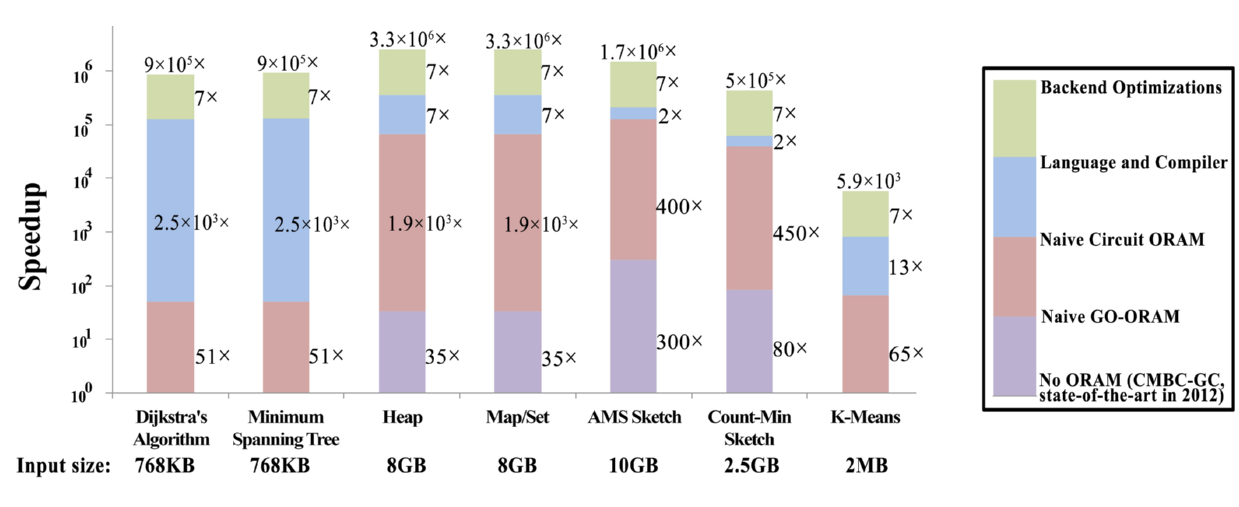
\includegraphics[width=1\textwidth]{speedup}
  \end{figure}
  \leftblock{20}{0}{0}{\LARGE{Thank You!}}

  \rightblock{20}{0}{0}{\color{blue}{\LARGE{http://oblivm.com/}}}

  \rightblock{20}{0}{2}{kartik@cs.umd.edu}
\end{frame}
\end{document}